\documentclass[letterpaper,twocolumn,openany]{dndarticle}

% Use babel or polyglossia to automatically redefine macros for terms
% Armor Class, Level, etc...
% Default output is in English; captions are located in lib/dndstring-captions.sty.
% If no captions exist for a language, English will be used.
%1. To load a language with babel:
%	\usepackage[<lang>]{babel}
%2. To load a language with polyglossia:
%	\usepackage{polyglossia}
%	\setdefaultlanguage{<lang>}
\usepackage[english]{babel}
%\usepackage[italian]{babel}
% For further options (multilanguage documents, hypenations, language environments...)
% please refer to babel/polyglossia's documentation.

\usepackage[utf8]{inputenc}
\usepackage[singlelinecheck=false]{caption}
\usepackage{lipsum}
\usepackage{listings}
\usepackage{shortvrb}
\usepackage{stfloats}
\usepackage{graphicx}
\usepackage{titling}
\usetikzlibrary{intersections} % Required for ornamentedtabular

\captionsetup[table]{labelformat=empty,font={sf,sc,bf,},skip=0pt}
\DndSetThemeColor[DmgLavender]

% Override the default background "paper" image with an alternate one.
\SetPaperImage{img/paper-article}

% The settings below are an example of how to modify all of the theme colors.
% Note that the paper (\SetPaperImage) and footerscroll.pdf will probably need
% to be modified for any major color scheme change. The values below are
% thematic for a sourcebook like GoS.
\definecolor {mytheme}      {HTML} {DCF1E5} %
\definecolor {mycomment}    {HTML} {E9F5F5} %
\definecolor {mysidebar}    {HTML} {E9F5F5} %
\definecolor {myreadaloud}  {HTML} {DCF1E5} %
\definecolor {myreadaloudborder}  {HTML} {8AA7A2} %
\definecolor {mypagenum}  {HTML} {B5D4CF} %
%\DndSetComplexThemeColor[mytheme][mycomment][mysidebar][myreadaloud][myreadaloudborder][titlered][titlegold][mypagenum]

\MakeShortVerb{|}

\lstset{%
  basicstyle=\ttfamily,
  language=[LaTeX]{TeX},
  breaklines=true,
}

\font\quipfont=cmr7 at 8pt
\title{An Authoritative Adventure}
\author{@author}
\date{{\quipfont \small\textit{A short quip that describes the adventure, such as ``Who will survive the attack of the murder-hobos?''}}}

% Adds an article image at the top of column 1 above the title, similar to the
% "Dungeon"-style article. Comment out the below to remove the image.
\pretitle{
  \Huge
  \vspace{-30pt} % Align top of image with column 2.
  \centering{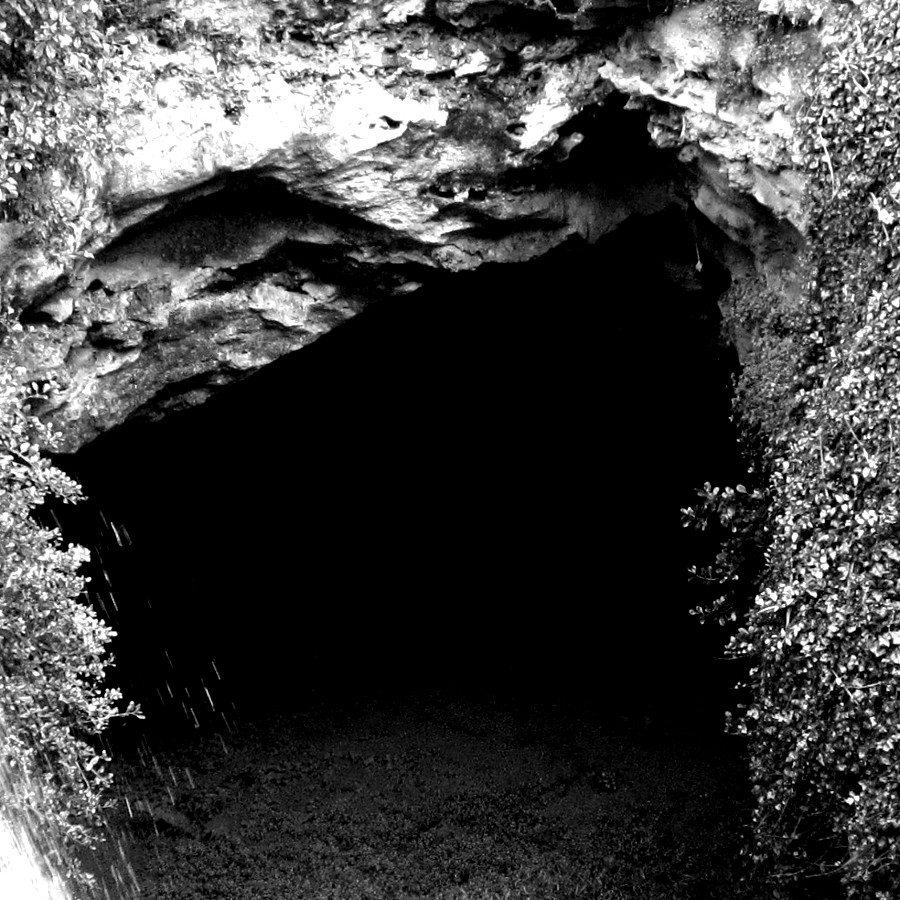
\includegraphics[width=7cm,height=7cm]{img/title.jpg}\\[\bigskipamount]}
  \begin{center}
}
\posttitle{\end{center}}

\begin{document}

\maketitle

\DndDropCapLine{T}{his package is designed to aid you in} writing beautifully typeset documents for the fifth edition of the world's greatest roleplaying game. It starts by adjusting the section formatting from the defaults in \LaTeX{} to something a bit more familiar to the reader. The article formatting is displayed above.

The default title layout is reminiscent of the article format in publications such as Dungeon magazine.

\section{Section}
Sections break up chapters into large groups of associated text.

\subsection{Subsection}
Subsections further break down the information for the reader.

\subsubsection{Subsubsection}
Subsubsections are the furthest division of text that still have a block header. Below this level, headers are displayed inline.

\paragraph{Paragraph}
The paragraph format is seldom used in the core books, but is available if you prefer the other style.

\subparagraph{Subparagraph}
The subparagraph format with the paragraph indent is likely going to be more familiar to the reader.

\subsubsection{Hanging Indent Features}
The |\listparagraph| format allows hanging indented
lists of options, such as those used for class features,
background skill/tool proficiency options, and
sometimes area features, for example:

\listparagraph[6pt]{Doors}
{The doors are made from thick lumber and are unlocked.}

\listparagraph{Light}
{The area is illuminated by candles placed in sconces on the
walls. Each candle has had a \textit{continual flame} spell
cast on it. Dispelling a flame is rumoured to give grievous offence
to the host.}

\listparagraph{Ventilation}
{All areas contain an adequate air supply. The air is renewed
via lung-like sacks that cling to the ceiling.}

\section{Special Sections}
The module also includes functions to aid in the proper typesetting of multi-line section headers: |\DndFeatHeader| for feats, |\DndItemHeader| magic items and traps, and |\DndSpellHeader| for spells.

\DndFeatHeader{Typesetting Savant}[Prerequisite: \LaTeX{} distribution]
You have acquired a package which aids in typesetting source material for one of your favorite games. You have advantage on Intelligence checks to typeset new content. On a failed check, you can ask questions online at the package's website.

\DndItemHeader{Foo's Quill}{Wondrous item, rare}
This quill has 3 charges. While holding it, you can use an action to expend 1 of its charges. The quill leaps from your hand and writes a contract applicable to your situation.

The quill regains 1d3 expended charges daily at dawn.

\DndSpellHeader%
  {Beautiful Typesetting}
  {4th-level illusion}
  {1 action}
  {5 feet}
  {S, M (ink and parchment, which the spell consumes)}
  {Until dispelled}
You are able to transform a written message of any length into a beautiful scroll. All creatures within range that can see the scroll must make a wisdom saving throw or be charmed by you until the spell ends.

While the creature is charmed by you, they cannot take their eyes off the scroll and cannot willingly move away from the scroll. Also, the targets can make a wisdom saving throw at the end of each of their turns. On a success, they are no longer charmed.

\subsection{Quotes}
\DndQuote%
  {``Sometimes, what you need and what you}
  {want turn out to be the same thing: An uplifting quote.''}
  {The Adventurer}

\section{Map Regions}
The map region functions |\area| and |\subarea| provide automatic numbering of areas.

\DndArea{Village of Hommlet}
This is the village of hommlet.

\DndSubArea{Inn of the Welcome Wench}
Inside the village is the inn of the Welcome Wench.

\DndSubArea{Blacksmith's Forge}
There's a blacksmith in town, too.

\DndArea{Foo's Castle}
This is foo's home, a hovel of mud and sticks.

\DndSubArea{Moat}
This ditch has a board spanning it.

\DndSubArea{Entrance}
A five-foot hole reveals the dirt floor illuminated by a hole in the roof.

\section{Alternate Map Region Styles}
Published modules sometimes use plain numbers for locations, sometimes plain
letters, and sometimes they prefix a character to the front of the numbers.
The following options can be used to display in these forms:

\numberedarea{Numbered Dungeon}
Areas in the Numbered Dungeon have sequential numbers. This is done using
the following commands:

\begin{verbatim}
\numberedarea{Numbered Dungeon}
\numberedsubarea{Entry}
\numberedsubarea{Trap}
\numberedsubarea{Fight}
\numberedsubarea{Exit}
\end{verbatim}

These commands yield the following results:
\numberedsubarea{Entry}
\numberedsubarea{Trap}
\numberedsubarea{Fight}
\numberedsubarea{Exit}

\letteredarea{Lettered Dungeon}
Areas in the Lettered Dungeon are labelled with sequential characters
(A, B, C, etc). This is done using the following commands:

\begin{verbatim}
\letteredarea{Lettered Dungeon}
\letteredsubarea{Entry}
\letteredsubarea{Trap}
\letteredsubarea{Fight}
\letteredsubarea{Exit}
\end{verbatim}

These commands yield the following results:
\letteredsubarea{Entry}
\letteredsubarea{Trap}
\letteredsubarea{Fight}
\letteredsubarea{Exit}

\prefixedarea{Prefixed Dungeon}{Z}
Areas in the Prefixed Dungeon have a custom prefix character,
in this case: `\prefixedareaprefix'.
This is done using the following commands:

\begin{verbatim}
\prefixedarea{Prefixed Dungeon}{Z}
\prefixedsubarea{Entry}
\prefixedsubarea{Trap}
\prefixedsubarea{Fight}
\prefixedsubarea{Exit}
\end{verbatim}

These commands yield the following results:
\prefixedsubarea{Entry}
\prefixedsubarea{Trap}
\prefixedsubarea{Fight}
\prefixedsubarea{Exit}

\section{Text Boxes}

The module has three environments for setting text apart so that it is drawn to the reader's attention. |DndReadAloud| is used for text that a game master would read aloud.

\begin{DndReadAloud}
  As you approach this module you get a sense that the blood and tears of many generations went into its making. A warm feeling welcomes you as you type your first words.
\end{DndReadAloud}

\subsection{As an Aside}
The other two environments are the |DndComment| and the |DndSidebar|. The |DndComment| is breakable and can safely be used inline in the text.

\begin{DndComment}{This Is a Comment Box!}
  A |DndComment| is a box for minimal highlighting of text. It lacks the ornamentation of |DndSidebar|, but it can handle being broken over a column.
\end{DndComment}

The |DndSidebar| is not breakable and is best used floated toward a page corner as it is below.

\begin{DndSidebar}[float=!b]{Behold the DndSidebar!}
  The |DndSidebar| is used as a sidebar. It does not break over columns and is best used with a figure environment to float it to one corner of the page where the surrounding text can then flow around it.
\end{DndSidebar}

\section{Tables}

\subsection{Regular Table}

The |DndTable| colors the even rows and is set to the width of a line by default.

\begin{DndTable}[header=Nice Table]{XX}
    Table head  & Table head \\
    Some value  & Some value \\
    Some value  & Some value \\
    Some value  & Some value
\end{DndTable}

The text in the first row of the table automatically uses boldface;
to prevent this, add ``bold=false'' to the optional parameters, for example:
\begin{lstlisting}[basicstyle=\ttfamily\small]
[header=Nice Table,bold=false]
\end{lstlisting}

\subsection{Alternate Table Background}

The |DndAltTable| allows tables that have a blank "header" line followed
by alternating theme color and white background, as per some of the sourcebooks.

\begin{DndAltTable}[header=Alternate Table,bold=false]{cX}
    \textbf{Table head} & \textbf{Table head} \\
    Some value  & Some value \\
    Some value  & Some value \\
    Some value  & Some value \\
    Some value  & Some value \\
\end{DndAltTable}

\subsection{Split Tables}
Temporarily adding a column using |multicols| can
be used to achieve the effect of a split column
table.

Add the following around two or more tables (note
the non-breaking space character (\char`\~) used for
the table header on all but the first):

\begin{lstlisting}[basicstyle=\ttfamily\small]
\begin{multicols}{2}
\begin{DndAltTable}[header=Encounters~(With~Spanning~Title)]{cX}
...
\end{DndAltTable}
\begin{DndAltTable}[header=~]{cX}
...
\end{DndAltTable}
\end{multicols}
\end{lstlisting}

This achieves the following effect:

\begin{multicols}{2}
\begin{DndAltTable}[header=Encounters~(With~Spanning~Title)]{cX}
    \textbf{d10} & \textbf{Encounter} \\
    1  & Toppled statue \\
    2  & Ferocious kitten \\
    3  & Broken sign \\
    4  & Blind beggar \\
    5  & Piercing wail \\
\end{DndAltTable}
\begin{DndAltTable}[header=~]{cX}
    \textbf{d10} & \textbf{Encounter} \\
    6  & Pack of wolves \\
    7  & Drunk owlbear \\
    8  & Freed prisoners \\
    9  & Wild magic zone \\
    10 & Magic item \\
\end{DndAltTable}
\end{multicols}

\subsection{Long Table that Spans Pages}

The |dndlongtable| allows table that can span multiple pages. The current
version is configured to do a two-column table.

\begin{dndlongtable}
    \textbf{Roll (d100)} & \textbf{Result} \\
    1-2 & You win a magic item or an expensive piece of classic artwork. \\
    3-4 & You win a magic item or an expensive piece of classic artwork. \\
    5-6 & You win a magic item or an expensive piece of classic artwork. \\
    7-8 & You win a magic item or an expensive piece of classic artwork. \\
    9-10 & You win a magic item or an expensive piece of classic artwork. \\
    11-12 & You win a magic item or an expensive piece of classic artwork. \\
    13-14 & You win a magic item or an expensive piece of classic artwork. \\
    15-16 & You win a magic item or an expensive piece of classic artwork. \\
    17-18 & You win a magic item or an expensive piece of classic artwork. \\
    19-20 & You win a magic item or an expensive piece of classic artwork. \\
    20-22 & You win a magic item or an expensive piece of classic artwork. \\
    23-24 & You win a magic item or an expensive piece of classic artwork. \\
    25-26 & You win a magic item or an expensive piece of classic artwork. \\
    27-28 & You win a magic item or an expensive piece of classic artwork. \\
    29-30 & You win a magic item or an expensive piece of classic artwork. \\
    31-32 & You win a magic item or an expensive piece of classic artwork. \\
    33-34 & You win a magic item or an expensive piece of classic artwork. \\
    35-36 & You win a magic item or an expensive piece of classic artwork. \\
    37-38 & You win a magic item or an expensive piece of classic artwork. \\
    39-40 & You win a magic item or an expensive piece of classic artwork. \\
    41-42 & You win a magic item or an expensive piece of classic artwork. \\
    43-44 & You win a magic item or an expensive piece of classic artwork. \\
    45-46 & You win a magic item or an expensive piece of classic artwork. \\
    47-48 & You win a magic item or an expensive piece of classic artwork. \\
    49-50 & You win a magic item or an expensive piece of classic artwork. \\
    51-52 & You win a magic item or an expensive piece of classic artwork. \\
    53-54 & You win a magic item or an expensive piece of classic artwork. \\
    55-56 & You win a magic item or an expensive piece of classic artwork. \\
    57-58 & You win a magic item or an expensive piece of classic artwork. \\
    59-60 & You win a magic item or an expensive piece of classic artwork. \\
    61-62 & You win a magic item or an expensive piece of classic artwork. \\
    63-64 & You win a magic item or an expensive piece of classic artwork. \\
    65-66 & You win a magic item or an expensive piece of classic artwork. \\
    67-68 & You win a magic item or an expensive piece of classic artwork. \\
    69-70 & You win a magic item or an expensive piece of classic artwork. \\
    71-72 & You win a magic item or an expensive piece of classic artwork. \\
    73-74 & You win a magic item or an expensive piece of classic artwork. \\
    75-76 & You win a magic item or an expensive piece of classic artwork. \\
    77-78 & You win a magic item or an expensive piece of classic artwork. \\
    79-80 & You win a magic item or an expensive piece of classic artwork. \\
    81 & You win a magic item or an expensive piece of classic artwork. \\
    82 & You win a magic item or an expensive piece of classic artwork. \\
    83 & You win a magic item or an expensive piece of classic artwork. \\
    84 & You win a magic item or an expensive piece of classic artwork. \\
    85 & You win a magic item or an expensive piece of classic artwork. \\
    86 & You win a magic item or an expensive piece of classic artwork. \\
    87 & You win a magic item or an expensive piece of classic artwork. \\
    88 & You win a magic item or an expensive piece of classic artwork. \\
    89 & You win a magic item or an expensive piece of classic artwork. \\
    90 & You win a magic item or an expensive piece of classic artwork. \\
    91 & You win a magic item or an expensive piece of classic artwork. \\
    92 & You win a magic item or an expensive piece of classic artwork. \\
    93 & You win a magic item or an expensive piece of classic artwork. \\
    94 & You win a magic item or an expensive piece of classic artwork. \\
    95 & You win a magic item or an expensive piece of classic artwork. \\
    96 & You win a magic item or an expensive piece of classic artwork. \\
    97 & You win a magic item or an expensive piece of classic artwork. \\
    98 & You win a magic item or an expensive piece of classic artwork. \\
    99 & You win a magic item or an expensive piece of classic artwork. \\
    100 & You win a magic item or an expensive piece of classic artwork. \\
\end{dndlongtable}

Since |dndlongtable| accepts column definitions in the standard |tabular|
format, alternate numbers of columns can be defined by passing an optional
parameter. For example, using:

\begin{lstlisting}[basicstyle=\ttfamily\small]
\begin{dndlongtable}[c p{0.66\linewidth} p{0.1\linewidth}]
\end{lstlisting}

Yields a three-column table:

\begin{dndlongtable}[c p{0.65\linewidth} p{0.12\linewidth}]
    \textbf{d100} & \textbf{Result} & \textbf{GP} \\
    1-2 & You win a magic item or an expensive piece of classic artwork. & 100 gp \\
    ... & & \\
    100 & You win a magic item or an expensive piece of classic artwork. & 1000 gp \\
\end{dndlongtable}

\subsection{Tables with Footnotes}
Surrounding one of the existing table types with a |minipage| section
allows footnotes declared in the table to appear at the end of the table,
rather than in the page footer as normal. For a regularly sized table
in the two-column layout, the following declaration can be used:

\begin{lstlisting}[basicstyle=\ttfamily\small]
\begin{minipage}{8cm}
  \begin{DndTable}
    ...
    ...
  \end{DndTable}
\end{minipage}
\end{lstlisting}

To achieve the following effect:

\begin{minipage}{8cm}
  \begin{DndTable}[header=Footnoted Table]{lX}
    \textbf{Table head\footnote{\enspace Something to note}} & \textbf{Table head} \\
    Some value  & Some value\footnote{\enspace Another thing to note} \\
    Some value  & Some value \\
    Some value  & Some value \\
    Some value\footnote{\enspace The most important note}  & Some value \\
  \end{DndTable}
\end{minipage}

\subsection{Ornamented Tables}
The |ornamentedtabular| allows tables similar to those used for spellcasters
(see over page).

\begin{figure*}[h!]
\begin{ornamentedtabular}{ccp{3.0cm}ccccccccccc}[title={The Full Caster}]
  & & & & & \multicolumn{9}{c}{\thead{--- Spell Slots per Spell Level ---}} \\
  \textbf{Level} & \textbf{\makecell{Proficiency\\Bonus}} & \textbf{Features} & \textbf{\makecell{Cantrips\\Known}} & \textbf{\makecell{Spells\\Known}} & \textbf{1st} & \textbf{2nd} & \textbf{3rd} & \textbf{4th} & \textbf{5th} & \textbf{6th} & \textbf{7th} & \textbf{8th} & \textbf{9th} \\
  1st  & +2 & Feature & 3 & 4  & 2 & — & — & — & — & — & — & — & — \\
  2nd  & +2 & Feature & 3 & 4  & 3 & — & — & — & — & — & — & — & — \\
  3rd  & +2 & Feature & 3 & 4  & 4 & 2 & — & — & — & — & — & — & — \\
  4th  & +2 & Feature & 4 & 5  & 4 & 3 & — & — & — & — & — & — & — \\
  5th  & +3 & Feature & 4 & 6  & 4 & 3 & 2 & — & — & — & — & — & — \\
  6th  & +3 & Feature & 4 & 7  & 4 & 3 & 3 & — & — & — & — & — & — \\
  7th  & +3 & Feature & 4 & 8  & 4 & 3 & 3 & 1 & — & — & — & — & — \\
  8th  & +3 & Feature & 4 & 9  & 4 & 3 & 3 & 2 & — & — & — & — & — \\
  9th  & +4 & Feature & 4 & 10 & 4 & 3 & 3 & 3 & 1 & — & — & — & — \\
  10th & +4 & Feature & 5 & 11 & 4 & 3 & 3 & 3 & 2 & — & — & — & — \\
  11th & +4 & Feature & 5 & 12 & 4 & 3 & 3 & 3 & 2 & 1 & — & — & — \\
  12th & +4 & Feature & 5 & 12 & 4 & 3 & 3 & 3 & 2 & 1 & — & — & — \\
  13th & +5 & Feature & 5 & 13 & 4 & 3 & 3 & 3 & 2 & 1 & 1 & — & — \\
  14th & +5 & Feature & 5 & 13 & 4 & 3 & 3 & 3 & 2 & 1 & 1 & — & — \\
  15th & +5 & Feature & 5 & 14 & 4 & 3 & 3 & 3 & 2 & 1 & 1 & 1 & — \\
  16th & +5 & Feature & 5 & 14 & 4 & 3 & 3 & 3 & 2 & 1 & 1 & 1 & — \\
  17th & +6 & Feature & 5 & 15 & 4 & 3 & 3 & 3 & 2 & 1 & 1 & 1 & 1 \\
  18th & +6 & Feature & 5 & 15 & 4 & 3 & 3 & 3 & 3 & 1 & 1 & 1 & 1 \\
  19th & +6 & Feature & 5 & 15 & 4 & 3 & 3 & 3 & 3 & 2 & 1 & 1 & 1 \\
  20th & +6 & Feature & 5 & 15 & 4 & 3 & 3 & 3 & 3 & 2 & 2 & 1 & 1 \\
\end{ornamentedtabular}
\end{figure*}

\clearpage

\section{Monsters and NPCs}
The |DndMonster| environment is used to typeset monster and NPC stat blocks. The module supplies many functions to easily typeset the contents of the stat block.

The stat block can be formatted either as a single column, or as a block that spans the page horizontally.

% Monster stat block
\begin{DndMonster}[float=h]{Monster Foo}
  \DndMonsterType{Medium aberration (metasyntactic variable), neutral evil}

  % If you want to use commas in the key values, enclose the values in braces.
  \DndMonsterBasics[
      armor-class = {9 (12 with \emph{mage armor})},
      hit-points  = {\DndDice{3d8 + 3}},
      speed       = {30 ft., fly 30 ft.},
    ]

  \DndMonsterAbilityScores[
      str = 12,
      dex = 8,
      con = 13,
      int = 10,
      wis = 14,
      cha = 15,
    ]

  \DndMonsterDetails[
      %saving-throws = {Str +0, Dex +0, Con +0, Int +0, Wis +0, Cha +0},
      %skills = {Acrobatics +0, Animal Handling +0, Arcana +0, Athletics +0, Deception +0, History +0, Insight +0, Intimidation +0, Investigation +0, Medicine +0, Nature +0, Perception +0, Performance +0, Persuasion +0, Religion +0, Sleight of Hand +0, Stealth +0, Survival +0},
      %damage-vulnerabilities = {cold},
      %damage-resistances = {bludgeoning, piercing, and slashing from nonmagical attacks},
      %damage-immunities = {poison},
      %condition-immunities = {poisoned},
      senses = {darkvision 60 ft., passive Perception 10},
      languages = {Common, Goblin, Undercommon},
      challenge = ---,
      proficiency = equals your bonus
    ]
  % Traits
  \DndMonsterAction{Innate Spellcasting}
  Foo's spellcasting ability is Charisma (spell save DC 12, +4 to hit with spell attacks). It can innately cast the following spells, requiring no material components:
  \begin{DndMonsterSpells}
    \DndInnateSpellLevel{misty step}
    \DndInnateSpellLevel[3]{fog cloud, rope trick}
    \DndInnateSpellLevel[1]{identify}
  \end{DndMonsterSpells}

  \DndMonsterAction{Spellcasting}
  Foo is a 2nd-level spellcaster. Its spellcasting ability is Charisma (spell save DC 12, +4 to hit with spell attacks). It has the following sorcerer spells prepared:
  \begin{DndMonsterSpells}
    \DndMonsterSpellLevel{blade ward, fire bolt, light, shocking grasp}
    \DndMonsterSpellLevel[1][3]{burning hands, mage armor, shield}
  \end{DndMonsterSpells}

  \DndMonsterSection{Actions}
  \DndMonsterAction{Multiattack}
  The foo makes two melee attacks.

  %Default values are shown commented out
  \DndMonsterAttack[
    name=Dagger,
    %distance=both, % valid options are in the set {both,melee,ranged},
    %type=weapon, %valid options are in the set {weapon,spell}
    mod=+3,
    %reach=5,
    %range=20/60,
    %targets=one target,
    dmg=\DndDice{1d4+1},
    dmg-type=piercing,
    %plus-dmg=,
    %plus-dmg-type=,
    %or-dmg=,
    %or-dmg-when=,
    %extra=,
  ]

  %\DndMonsterMelee calls \DndMonsterAttack with the melee option
  \DndMonsterMelee[
    name=Flame Tongue Longsword,
    mod=+3,
    %reach=5,
    %targets=one target,
    dmg=\DndDice{1d8+1},
    dmg-type=slashing,
    plus-dmg=\DndDice{2d6},
    plus-dmg-type=fire,
    or-dmg=\DndDice{1d10+1},
    or-dmg-when=if used with two hands,
    %extra=,
  ]

  %\DndMonsterRanged calls \DndMonsterAttack with the ranged option
  \DndMonsterRanged[
    name=Assassin's Light Crossbow,
    mod=+1,
    range=80/320,
    dmg=\DndDice{1d8},
    dmg-type=piercing,
    %plus-dmg=,
    %plus-dmg-type=,
    %or-dmg=,
    %or-dmg-when=,
    extra={, and the target must make a DC 15 Constitution saving throw, taking 24 (7d6) poison damage on a failed save, or half as much damage on a successful one}
  ]

  % Legendary Actions
  \DndMonsterSection{Legendary Actions}
  The foo can take 3 legendary actions, choosing from the options below. Only one legendary action option can be used at a time and only at the end of another creature's turn. The foo regains spent legendary actions at the start of its turn.

  \begin{DndMonsterLegendaryActions}
    \DndMonsterLegendaryAction{Move}{The foo moves up to its speed.}
    \DndMonsterLegendaryAction{Dagger Attack}{The foo makes a dagger attack.}
    \DndMonsterLegendaryAction{Create Contract (Costs 3 Actions)}{The foo presents a contract in a language it knows and waves it in the face of a creature within 10 feet. The creature must make a DC 10 Intelligence saving throw. On a failure, the creature is incapacitated until the start of the foo's next turn. A creature who cannot read the language in which the contract is written has advantage on this saving throw.}
  \end{DndMonsterLegendaryActions}
\end{DndMonster}

% Monster stat block
\begin{DndMonster}[float*=b,width=\textwidth + 8pt]{Monster Foo}
  \begin{multicols}{2}
    \DndMonsterType{Medium aberration (metasyntactic variable), neutral evil}

    % If you want to use commas in the key values, enclose the values in braces.
    \DndMonsterBasics[
        armor-class = {9 (12 with \emph{mage armor})},
        hit-points  = {\DndDice{3d8 + 3}},
        speed       = {30 ft., fly 30 ft.},
      ]

    \DndMonsterAbilityScores[
        str = 12,
        dex = 8,
        con = 13,
        int = 10,
        wis = 14,
        cha = 15,
      ]

    \DndMonsterDetails[
        %saving-throws = {Str +0, Dex +0, Con +0, Int +0, Wis +0, Cha +0},
        %skills = {Acrobatics +0, Animal Handling +0, Arcana +0, Athletics +0, Deception +0, History +0, Insight +0, Intimidation +0, Investigation +0, Medicine +0, Nature +0, Perception +0, Performance +0, Persuasion +0, Religion +0, Sleight of Hand +0, Stealth +0, Survival +0},
        %damage-vulnerabilities = {cold},
        %damage-resistances = {bludgeoning, piercing, and slashing from nonmagical attacks},
        %damage-immunities = {poison},
        %condition-immunities = {poisoned},
        senses = {darkvision 60 ft., passive Perception 10},
        languages = {Common, Goblin, Undercommon},
        challenge = 1,
        proficiency = +2,
      ]
    % Traits
    \DndMonsterAction{Innate Spellcasting}
    Foo's spellcasting ability is Charisma (spell save DC 12, +4 to hit with spell attacks). It can innately cast the following spells, requiring no material components:
    \begin{DndMonsterSpells}
      \DndInnateSpellLevel{misty step}
      \DndInnateSpellLevel[3]{fog cloud, rope trick}
      \DndInnateSpellLevel[1]{identify}
    \end{DndMonsterSpells}

    \DndMonsterAction{Spellcasting}
    Foo is a 2nd-level spellcaster. Its spellcasting ability is Charisma (spell save DC 12, +4 to hit with spell attacks). It has the following sorcerer spells prepared:
    \begin{DndMonsterSpells}
      \DndMonsterSpellLevel{blade ward, fire bolt, light, shocking grasp}
      \DndMonsterSpellLevel[1][3]{burning hands, mage armor, shield}
    \end{DndMonsterSpells}

    \DndMonsterSection{Actions}
    \DndMonsterAction{Multiattack}
    The foo makes two melee attacks.

    %Default values are shown commented out
    \DndMonsterAttack[
      name=Dagger,
      %distance=both, % valid options are in the set {both,melee,ranged},
      %type=weapon, %valid options are in the set {weapon,spell}
      mod=+3,
      %reach=5,
      %range=20/60,
      %targets=one target,
      dmg=\DndDice{1d4+1},
      dmg-type=piercing,
      %plus-dmg=,
      %plus-dmg-type=,
      %or-dmg=,
      %or-dmg-when=,
      %extra=,
    ]

    %\DndMonsterMelee calls \DndMonsterAttack with the melee option
    \DndMonsterMelee[
      name=Flame Tongue Longsword,
      mod=+3,
      %reach=5,
      %targets=one target,
      dmg=\DndDice{1d8+1},
      dmg-type=slashing,
      plus-dmg=\DndDice{2d6},
      plus-dmg-type=fire,
      or-dmg=\DndDice{1d10+1},
      or-dmg-when=if used with two hands,
      %extra=,
    ]

    %\DndMonsterRanged calls \DndMonsterAttack with the ranged option
    \DndMonsterRanged[
      name=Assassin's Light Crossbow,
      mod=+1,
      range=80/320,
      dmg=\DndDice{1d8},
      dmg-type=piercing,
      %plus-dmg=,
      %plus-dmg-type=,
      %or-dmg=,
      %or-dmg-when=,
      extra={, and the target must make a DC 15 Constitution saving throw, taking 24 (7d6) poison damage on a failed save, or half as much damage on a successful one}
    ]

    % Legendary Actions
    \DndMonsterSection{Legendary Actions}
    The foo can take 3 legendary actions, choosing from the options below. Only one legendary action option can be used at a time and only at the end of another creature's turn. The foo regains spent legendary actions at the start of its turn.

    \begin{DndMonsterLegendaryActions}
      \DndMonsterLegendaryAction{Move}{The foo moves up to its speed.}
      \DndMonsterLegendaryAction{Dagger Attack}{The foo makes a dagger attack.}
      \DndMonsterLegendaryAction{Create Contract (Costs 3 Actions)}{The foo presents a contract in a language it knows and waves it in the face of a creature within 10 feet. The creature must make a DC 10 Intelligence saving throw. On a failure, the creature is incapacitated until the start of the foo's next turn. A creature who cannot read the language in which the contract is written has advantage on this saving throw.}
    \end{DndMonsterLegendaryActions}
  \end{multicols}
\end{DndMonster}

\clearpage

\section{Colors}

\begin{table*}[b]%
  \begin{DndTable}[width=\linewidth,header=Colors Supported by This Package]{lX}
    \textbf{Color}                  & \textbf{Description} \\
    \rowcolor{PhbLightGreen}
    |PhbLightGreen|                 & Light green used in PHB Part 1 (Default) \\
    \rowcolor{PhbLightCyan}
    |PhbLightCyan|                  & Light cyan used in PHB Part 2 \\
    \rowcolor{PhbMauve}
    |PhbMauve|                      & Pale purple used in PHB Part 3 \\
    \rowcolor{PhbTan}
    |PhbTan|                        & Light brown used in PHB appendix \\
    \rowcolor{DmgLavender}
    |DmgLavender|                   & Pale purple used in DMG Part 1 \\
    \rowcolor{DmgCoral}
    |DmgCoral|                      & Orange-pink used in DMG Part 2 \\
    \rowcolor{DmgSlateGray}
    |DmgSlateGray| (|DmgSlateGrey|) & Blue-gray used in DMG Part 3 \\
    \rowcolor{DmgLilac}
    |DmgLilac|                      & Purple-gray used in DMG appendix \\
    \rowcolor{BrGreen}
    |BrGreen|                       & Light-gray used for tables in Basic Rules\\
  \end{DndTable}
\end{table*}

This package provides several global color variables to style |DndComment|, |DndReadAloud|, |DndSidebar|, and |DndTable| environments.

\begin{DndTable}[header=Box Colors]{lX}
  \textbf{Color}   & \textbf{Description} \\
  |commentcolor|   & |DndComment| background \\
  |readaloudcolor| & |DndReadAloud| background \\
  |sidebarcolor|   & |DndSidebar| background \\
  |tablecolor|     & background of even |DndTable| rows \\
\end{DndTable}

They also accept an optional color argument to set the color for a single instance. See Table~\ref{tab:colors} for a list of core book accent colors.

\begin{lstlisting}[basicstyle=\ttfamily\small]
\begin{DndTable}[cX][PhbLightCyan]
  \textbf{d8} & \textbf{Item} \\
  1           & Small wooden button \\
  2           & Red feather \\
  3           & Human tooth \\
  4           & Vial of green liquid \\
  5           & Loaded dice \\
  6           & Tasty biscuit \\
  7           & Broken axe handle \\
  8           & Tarnished silver locket \\
\end{DndTable}
\end{lstlisting}

\begin{DndTable}[color=PhbLightCyan]{cX}
  \textbf{d8} & \textbf{Item} \\
  1           & Small wooden button \\
  2           & Red feather \\
  3           & Human tooth \\
  4           & Vial of green liquid \\
  5           & Loaded dice \\
  6           & Tasty biscuit \\
  7           & Broken axe handle \\
  8           & Tarnished silver locket \\
\end{DndTable}

\subsection{Themed Colors}
Use |\DndSetThemeColor[<color>]| to set |commentcolor|, |readaloudcolor|, |sidebarcolor|, and |tablecolor| to a specific color. Calling |\DndSetThemeColor| without an argument sets those colors to the current |themecolor|. In the following example the group limits the change to just a few boxes; after the group finishes, the colors are reverted to what they were before the group started.

\begin{lstlisting}[basicstyle=\ttfamily\small]
\begingroup
\DndSetThemeColor[PhbMauve]

\begin{DndComment}{This Comment Is in Mauve}
  This comment is in the the new color.
\end{DndComment}

\begin{DndSidebar}{This Sidebar Is Also Mauve}
  The sidebar is also using the new theme color.
\end{DndSidebar}
\endgroup
\end{lstlisting}

\begingroup
\DndSetThemeColor[PhbMauve]

\begin{DndComment}{This Comment Is in Mauve}
  This comment is in the the new color.
\end{DndComment}

\begin{DndSidebar}{This Sidebar Is Also Mauve}
  The sidebar is also using the new theme color.
\end{DndSidebar}

\endgroup

\subsection{Extra Theme Color Control}
Use |\DndSetComplexThemeColor| in order to have more precise control over the various theme colors defined within the document class. This command takes eight (8) |<color>| values that map to the following color variables within the theme:

\begin{DndTable}[header=Complex Theme Parameter Map]{clX}
  \textbf{\#} & \textbf{Variable Set} & \textbf{Affected Style} \\
  1 & \textit{themecolor} & Used in |DndSetThemeColor|; set for future compatibility \\
    & \textit{tablecolor} & |DndTable| \\
  2 & \textit{commentcolor} & |DndComment| \\
  3 & \textit{sidebarcolor} & |DndSidebar| \\
  4 & \textit{readaloudcolor} & |DndReadAloud| background \\
  5 & \textit{readaloudbordercolor} & |DndReadAloud| border \\
  6 & \textit{titlecolor} & Titles of sections (|section|, |subsection|, etc) \\
  7 & \textit{titlerulecolor} & |subsection| title ruling \\
  8 & \textit{pagecolor} & Page numbers and footer \\
\end{DndTable}

\begin{DndComment}{Note On Changing Schemes}
If a major color scheme change is attempted, it is
likely that the background ``paper'' (which can be overridden with
|\SetPaperImage|) and footerscroll.pdf will need
to be modified as well in order to fit the other color modifications.
\end{DndComment}

An example of these settings for a theme similar to the \textit{Ghosts of Saltmarsh} sourcebook. Note that the values for \textit{titlered} and \textit{titlegold} are used for the title and title rule colours unchanged in this example.

\begin{lstlisting}[basicstyle=\ttfamily\small]
\definecolor {mytheme} {HTML} {DCF1E5}
\definecolor {mycomment} {HTML} {E9F5F5}
\definecolor {mysidebar} {HTML} {E9F5F5}
\definecolor {myreadaloud} {HTML} {DCF1E5}
\definecolor {myreadaloudborder} {HTML} {8AA7A2}
\definecolor {mypagenum} {HTML} {B5D4CF}
\DndSetComplexThemeColor[mytheme][mycomment][mysidebar][myreadaloud][myreadaloudborder][titlered][titlegold][mypagenum]
\end{lstlisting}

\end{document}
